\section{Experiments\label{sec:experiment}}

\subsection{Experiments on Finding the Best Iterative Trail}

We apply our method in Section \ref{sec:fbit} to PRESENT, GIFT-64, RECTANGLE, 256-bit KNOT permutation and ASCON permutation. The results on the best iterative trail are shown in Table \ref{tab:it}. The visualizations of $G^{IS}_{F,max\_asn}$ are shown in Appendix \ref{app:visualization}. These results are not improved by the technique in Section \ref{sec:expansion}

\begin{table}
	\caption{Results on the weight growth of one best single iterative trail}\label{tab:it}
	\centering
	\begin{tabular}{|c|c|c|c|c|}
		\hline
		cryptanalysis & cipher & $max\_asn$ & $-\log_2(wt)/rd$\\
		\hline
		diff. & 256-bit KNOT permutation & 2 & 5.3\\
		\hline
		diff. & PRESENT & 2 & 4.5\\
		\hline
		diff. & GIFT-64 & 2 & 5\\
		\hline
		diff. & RECTANGLE & 2 & 5\\
		\hline
		diff. & ASCON permutation & 3 & -\\
		\hline
		linear & 256-bit KNOT permutation & 2 & 6*\\
		\hline
		linear & PRESENT & 1 & 4\\
		\hline
		linear & GIFT-64 & 2 & 6\\
		\hline
		linear & RECTANGLE & 2 & 6\\
		\hline
		linear & ASCON permutation & 3 & -\\
		\hline
	\end{tabular}
\end{table}

Note that for 256-bit KNOT permutation has no key addition, the weight of the linear trail we compute is the correlation of the linear trail instead of the correlation square averaging on round keys for block ciphers. To fairly compare the result of the best linear trail of 256-bit KNOT permutation with other ciphers, we square its correlation.

For ASCON permutation, we set $max\_asn$ to 3 and find no iterative trail though the generated graph is not empty. 

Among other ciphers which we experiment on, we find that 256-bit KNOT permutation has the smallest differential probability growth of the best single differential iterative trail, while PRESENT has the largest. And also PRESENT has the largest linear correlation growth of the best single linear iterative trail, while the other three have the same. 

\subsection{Experiments on Finding the Best Iterative Hull}

We apply our method in Section \ref{sec:fbih} to PRESENT, GIFT-64, RECTANGLE, 256-bit KNOT permutation. And we generate $G_{F,T_{a,b,c}}$ using the technique in Section \ref{sec:expansion} instead of generating $G_{F,max\_asn}$. In case of linear cryptanalysis of PRESENT, the parameters $(a,b,c)$ is set to (1,2,3). In other cases, $(a,b,c)$ is set to (2,3,3).

The results on the best iterative hull according to a given number of rounds are shown in Figure \ref{fig:plot_ih}. The number of rounds is denoted as $rd$ which is the x axis of Figure \ref{fig:plot_ih}. The weight of the best iterative hull is denoted as $wt$ and the y axis of Figure \ref{fig:plot_ih} is $-\log_2(wt)/rd$ which describes the weight growth. 

\begin{figure}
	\centering
	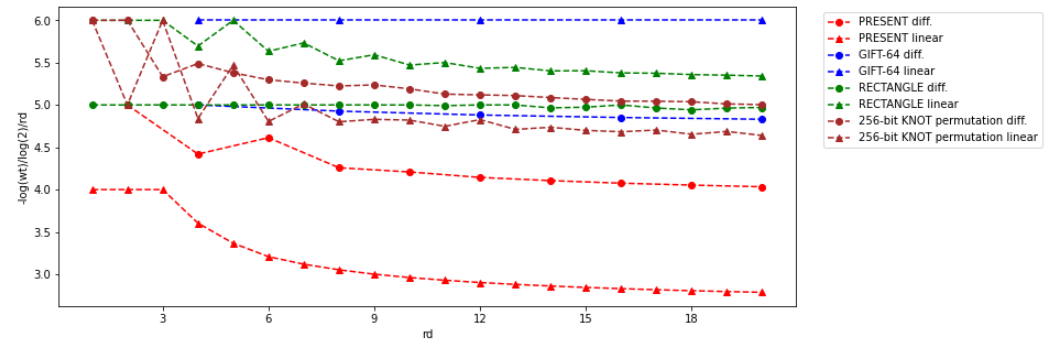
\includegraphics[width=1\textwidth]{fig/plot_iterative_hulls.PNG}
	\caption{Results on the weight growth of the best iterative hull} \label{fig:plot_ih}
\end{figure}

For any cipher we conduct experiments on, the weight growth of iterative hulls is larger than the weight growth of iterative trails except for the case of linear cryptanalysis of GIFT-64. In most cases with the given number of round $rd$ increasing, we observe that the weight per round of the best iterative hull increases (its negative logrithm decreases). This implies that the combination of iterative trails enhances differential and linear propagations. 


%We consider the smallest weight per length an elementary iterative trail can has (best w/l. in Table \ref{tab:iterative-trails}) as an index describing the growth of iterative differential and linear propagations. We can see that PRESENT has both the weakest growth of iterative differential and linear propagations. The weakest differential iterative trail is exactly the one found by Wang et al.\cite{W08}. 

%256-bit KNOT permutation, PRESENT, GIFT-64 and RECTANGLE share a common point that each of them uses a bit permutation as its linear layer which is hardware-friendly and an S-box also providing diffusion as its non-linear layer. However, due to the weakness of the linear layer, the best differential and linear weights of them all increase proportionally with the round number, because of the existence of iterative trails. Meanwhile ASCON permutation uses a low-latency S-box and a strong linear layer. From Table \ref{tab:is} we can see that the differential iterative structure of ASCON permutation is empty even when $k=3$.

%A question is raised that how far a cipher with a comparatively weak diffusion layer can go. As long as the iterative structure is not empty, the best weight increases proportionally with the round number. Through the visualization of iterative structure, we hope to inform symmetric-key primitive designers of the detailed structure of iterative trails. 

%\subsection{Results of the Best Weights}
%
%Results for 256-bit KNOT permutation, PRESENT, GIFT-64 and RECTANGLE on the best weights obtained using our methods in section \ref{sec:para2} and \ref{sec:para3} are illustrated in Tables \ref{tab:knot256}-\ref{tab:rect}. They are compared with the weights of the best differential and linear trails. Using the method proposed in section \ref{sec:para2}, we need to determine the parameters $(r^f,r^b)$ first. Using the method proposed in section \ref{sec:para3}, we need to determine the parameters $(r^f,w^f,r^b,w^b,gap)$ first, where $gap=wub-bw[r]$ when searching $r$-round clusters. The larger each parameter is, the more time is consumed and the more accurate the result is. 
%
%The results obtained by our method coincide with the results of genuine best weight when the round number is large, except for results of linear weights for GIFT-64. The best 13-round linear trail of GIFT given in \cite{ZZDX19} has correlation $2^{-34}$ and has no iterative trail in it. Our method is unable to find such a trail. 
%
%%Our method finishes in minutes or even in seconds and is able to obtain an upper bound of the best weight for ciphers have iterative trails.

\subsection{Experiments on Estimating EDPs and ELPs}

We apply our method in Section \ref{sec:fbh} to PRESENT, GIFT-64, RECTANGLE and 256-bit KNOT permutation. The algorithm is run on an Intel Core i7-6700 CPU at 3.40GHz with 16GB RAM. The results for differential cryptanalysis are shown in Table \ref{tab:EDP}. The results for linear cryptanalysis are shown in Table \ref{tab:ELP}. 

Same as the work in \cite{HV18}, we use a multistage graph method to find good differentials and linear hulls. But our method is motivated by iterative trails and has a different routine of choosing the interesting subgraph. Results for PRESENT, RECTANGLE and GIFT-64 are close to the results in \cite{HV18}, which implies that iterative trails dominate the good differentials and linear hulls of these ciphers. Our method costs much less time. For RECTANGLE, we improve the 14-round ELP to $2^{-62.31}$. 

The 256-bit KNOT permutation is used in NIST LWC round 2 candidate KNOT \cite{ZDY19}, which is an inheritor of RECTANGLE having a larger number of rounds and a larger block size. For the 256-bit KNOT permutation, we are able to find good differentials up to 52 rounds and good linear hulls up to 51 rounds, while the best single differential trail is found up to 48 rounds and the best single linear trail is found up to 44 rounds according to the specification document of KNOT \cite{ZDY19}. 

\begin{table}
	\caption{Results on estimating EDPs}\label{tab:EDP}
	\centering
	\begin{tabular}{|c|c|c|c|c|c|c|}
		\hline
		cipher & rd & $(a,b,c)$ & $(k,-\log_2wlb)$ & $-\log_2\Prob$ & $-\log_2\EDP$ & Time \\
		\hline
		PRESENT & 16 & (2,3,3) & (3,10) & 70 & 61.84 & 26s+165s\\
		\hline
		GIFT-64 & 13 & (2,3,3) & (3,13) & 62 & 60.42 & 24s+76s\\
		\hline 
		RECTANGLE & 14 & (2,*,1) & (6,25) &  &  &  \\
		\hline
		KNOT-perm-256 & 52 & (2,*,1) & (3,12) & 274 & 251.831 & 0s+10s\\
		\hline
	\end{tabular}
\end{table}

\begin{table}
	\caption{Results on estimating ELPs}\label{tab:ELP}
	\centering
	\begin{tabular}{|c|c|c|c|c|c|c|}
		\hline
		cipher & rd & $(a,b,c)$ & $(k,-\log_2wlb)$ & $-2\log_2\Cor$ & $-\log_2\ELP$ & Time \\
		\hline
		PRESENT & 24 & (1,2,3) & (3,8) & 92 & 63.61 & 0s+14s\\
		\hline
		GIFT-64 & 13 & (2,*,1) & (3,10) & 64 & 64 & 1s+1s\\
		\hline 
		RECTANGLE & 14 & (2,3,3) & (3,14) & 68 & 62.31 & 17s+5433s \\
		\hline
		KNOT-perm-256 & 52 & (2,3,3) & (2,6) &  &  & \\
		\hline
	\end{tabular}
\end{table}



\subsection{Experiment on KNOT}

KNOT is a family of lightweight authenticated encryption algorithms and hash functions \cite{ZDY19}. The modes of operation of KNOT for AE and hash are shown in Figure . The modes are similar to the ones used in Ketje and ASCON. The inner permutations are inheritors of RECTANGLE, which are bit-sliced lightweight. The round transformation has 3 steps: 4-bit S-boxes, row rotations and a constant addition. The operation modes of AEAD and Hash are shown in 

\begin{figure}
	\centering
	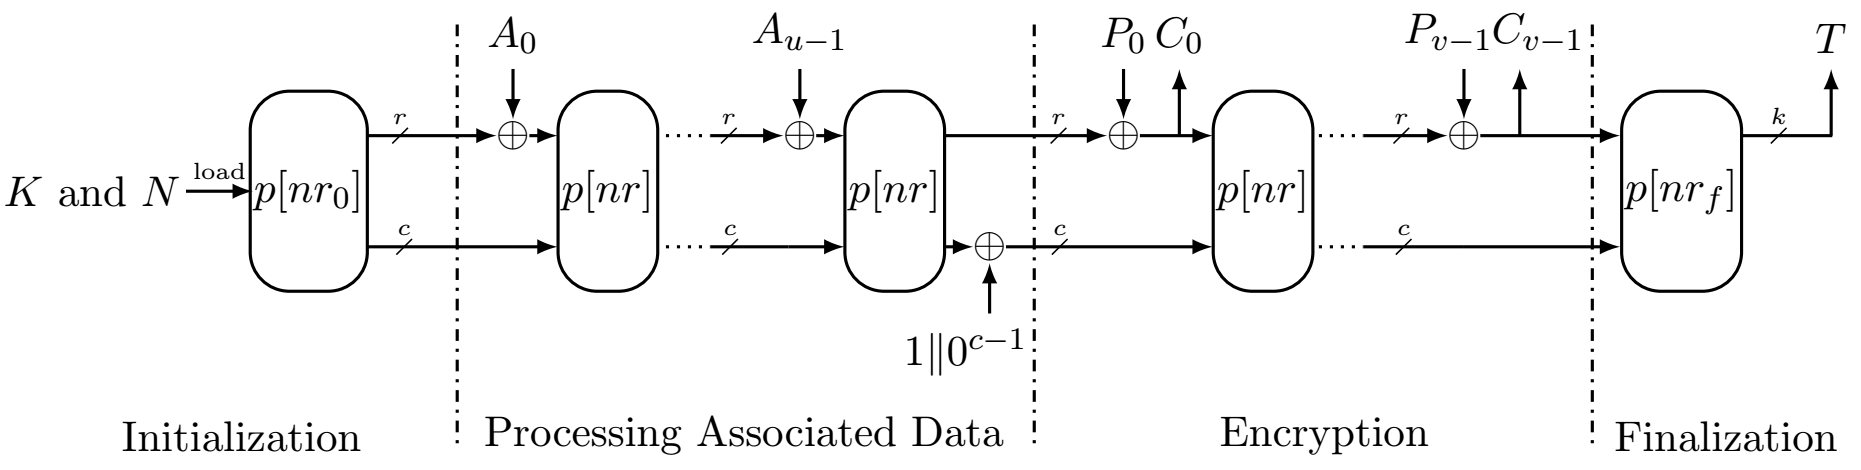
\includegraphics[width=1\textwidth]{fig/mode_aead.PNG}
	\caption{The operation mode of KNOT AEAD} \label{fig:mode_aead}
\end{figure}

\begin{figure}
	\centering
	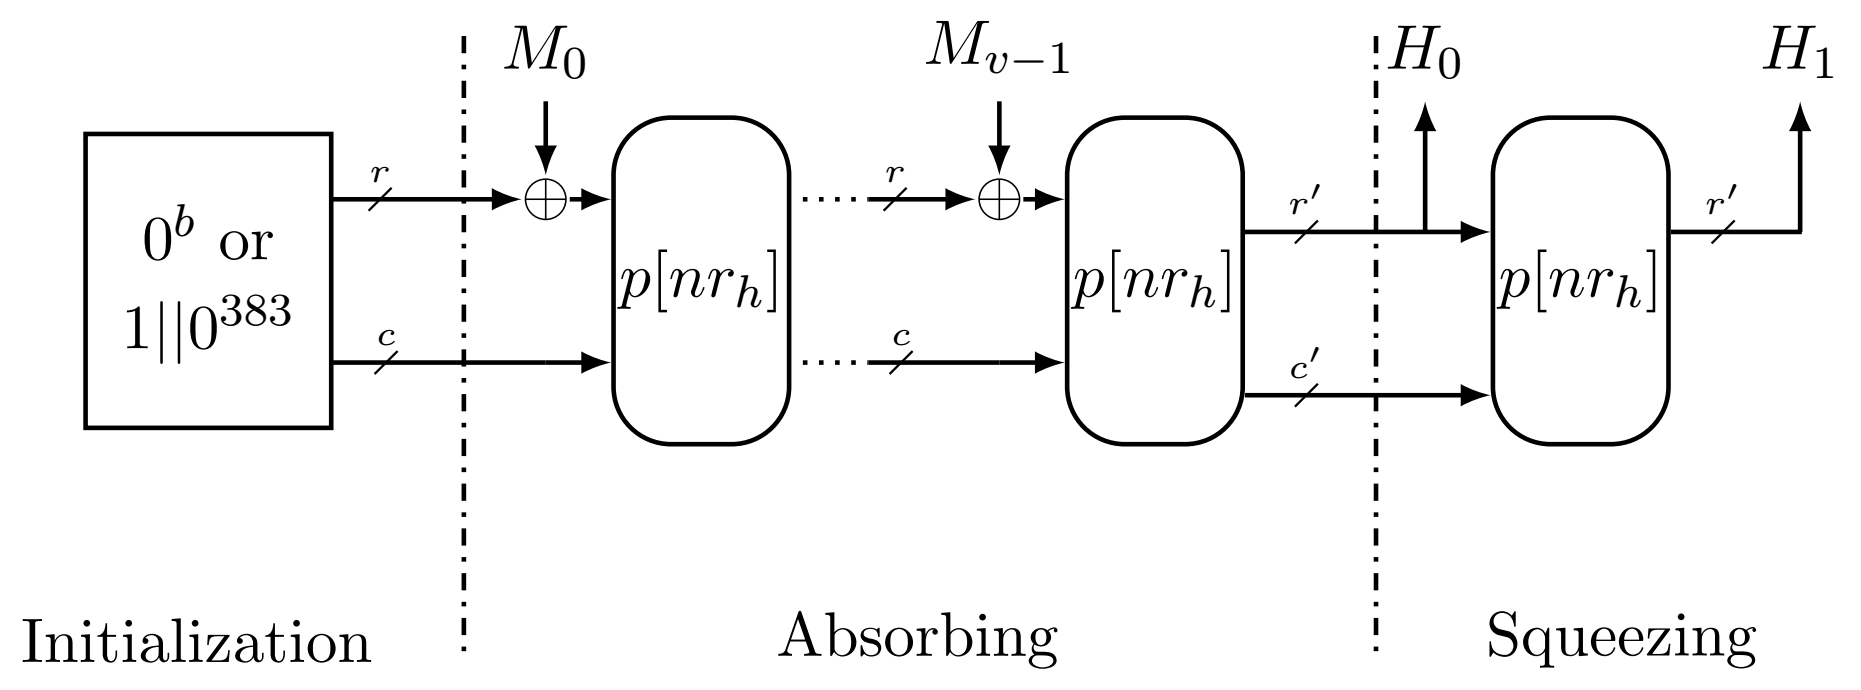
\includegraphics[width=0.7\textwidth]{fig/mode_hash.PNG}
	\caption{The operation mode of KNOT Hash} \label{fig:mode_hash}
\end{figure}

In the original specification document of KNOT, The largest differential probability and linear correlation is given. However firstly, the differential and linear distinguishers with no restrictions can not be directly uesd to attack the MonkeyDuplex construction. Secondly, the clustering effect is not taken into consideration. Thirdly, because only the rate part and the tag part is visible, differences can be truncated in the capacity part and in the non-tag part. 

In the following, we propose differential and linear attacks targeting different phases, each demanding specific restrictions on the distinguishers. The attacks proposed are general for cryptographic schemes based on MonkeyDuplex construction. For each attack, we give the largest differential probability or linear correlation square of the longest distinguisher as in Table \ref{tab:knot}. 

\subsubsection{Attack Model 1}
This is a chosen-nonce differential distinguishing attack targeting the initialization phase of KNOT-AEAD. The input difference has the nonce part and key part $\Delta SI=(\Delta SI_N,\Delta SI_K)$. The output difference has the rate part and capacity part $\Delta SO=(\Delta SO_R,\Delta SO_C)$. We restrict that $\Delta SI_K=0$. And $\Delta SO_C$ is truncated. 

\subsubsection{Attack Model 2}
This is a known-nonce and known-plaintext linear key recovery attack targeting the initialization phase of KNOT-AEAD. The input mask $\Gamma SI=(\Gamma SI_N,\Gamma SI_K)$ and the output mask $\Gamma SO=(\Gamma SO_R,\Gamma SO_C)$. We restrict that $\Gamma SO_C=0$. Note that if for the best linear distinguisher $\Gamma SI_K\neq 0$, then the attack degrades to a distinguishing one, which is however very unlikely. 

%\subsubsection{Attack Model 3}
%This is a known-nonce and known-plaintext linear distinguishing attack targeting the initialization phase of KNOT-AEAD in multi-key setting. The input mask $\Gamma SI=(\Gamma SI_N,\Gamma SI_K)$ and the output mask $\Gamma SO=(\Gamma SO_R,\Gamma SO_C)$. We restrict that $\Gamma SO_C=0$ and $\Gamma SI_K=0$.

\subsubsection{Attack Model 3}
This is a known-plaintext linear distinguishing attack targeting the encryption phase of KNOT-AEAD. The input mask $\Gamma SI=(\Gamma SI_R,\Gamma SI_C)$ and the output mask $\Gamma SO=(\Gamma SO_R,\Gamma SO_C)$. We restrict that $\Gamma SI_C=0$ and $\Gamma SO_C=0$. 


\subsubsection{Attack Model 4}
This is a differential forgery attack targeting the encryption phase of KNOT-AEAD. The input difference $\Delta SI=(\Delta SI_R,\Delta SI_C)$ and the output difference $\Delta SO=(\Delta SO_R,\Delta SO_C)$. We restrict that $\Delta SI_C=0$ and $\Delta SO_C=0$. 

\subsubsection{Attack Model 5}
This is a differential forgery attack targeting the finalization phase of KNOT-AEAD. The input difference $\Delta SI=(\Delta SI_R,\Delta SI_C)$ and the output difference $\Delta SO=(\Delta SO_T,\Delta SO_{nT})$. We restrictions that $\Delta SI_C=0$. And $\Delta SO_{nT}$ is truncated. 



\subsubsection{Attack Model 6}
This is a differential collsion attack targeting the absorb phase of KNOT-Hash. The input difference $\Delta SI=(\Delta SI_R,\Delta SI_C)$ and the output difference $\Delta SO=(\Delta SO_R,\Delta SO_C)$. We restrictions that $\Delta SI_C=0$ and $\Delta SO_C=0$. 

\subsubsection{Attack Model 7}
This is a differential collsion attack targeting the squeezing phase of KNOT-Hash. The input difference $\Delta SI=(\Delta SI_R,\Delta SI_C)$ and the output difference $\Delta SO=(\Delta SO_{R'},\Delta SO_{C'})$. We restrictions that $\Delta SI_C=0$ and $\Delta SI_{R'}=0$. And $\Delta SI_{C'}$ is truncated. 

\begin{table}
	\caption{Results for the primary version of KNOT}\label{tab:knot}
	\centering
	\begin{tabular}{|c|c|c|c|c|c|c|c|}
		\hline
		Attack Model & rounds & $(a,b,c)$ & $(k,-\log_2wlb)$ & $-\log_2$(EDP or ELP)\\
		\hline
		AM1 & 14 & (2,*,1) & (5,20) & 62.2 \\
		AM2 & 13 & (2,3,3) & (3,8) & 30.7*2=61.4 \\
		AM3 & 12 & (2,3,3) & (3,10) & 30.2*2=60.4 \\
		AM4 & 12 & (2,*,1) & (5,20) & 62.4 \\
		AM5 & 13 & (2,*,1) & (5,20) & 61.4 \\
		AM6 & 12 & (2,*,1) & (5,20) & 62.7 \\
		AM7 & 13 & (2,*,1) & (5,20) & 61.4 \\
		\hline
	\end{tabular}
\end{table}

\subsubsection{Summary}

The results in Table \ref{tab:knot} show that the inner permutations in the initialization, encryption and finalization phases of the primary version of KNOT-AEAD should have more than 14 rounds, 12 rounds and 13 rounds respectively. The inner permutations in the absorbing and squeezing phases of the primary version of KNOT-Hash should have more than 12 rounds and 13 rounds. 

